\documentclass{beamer}
\usepackage{ifpdf}
\usepackage{grffile}
\usepackage{epsfig} % This package formats figures.
\usepackage{psfrag} % This package formats figures.
\usepackage{amsmath} % This is a package for math features.
\usepackage{amsfonts} % This is a package for math features.
\usepackage{amssymb} % This is a package for math features.
\usepackage{graphicx}
\usepackage{epstopdf}


\usetheme{CambridgeUS}
\begin{document}

\title[Probabilistic Networks]{Networks with Probabilistic Failures}
\subtitle[Probabilistically Scoring Message Priorities]{Scoring Message Priorities in Switched Networks with Probabilistic Failures}
\author[Shubham Goel]{Shubham Goel \inst{1}, Guillermo Navas-Rodriguez \inst{2}, Guy Avni \inst{3} and Thomas Henzinger \inst{3}}
\institute[IIT Bombay]{
  \inst{1} Indian Institute of Technology, Bombay\\
  \inst{2} Malardalen University, Sweden\\
  \inst{3} IST Austria\\[1ex]
}
\date[Summer 2016]{Summer 2016}

\begin{frame}[plain]
  \titlepage
\end{frame}

\begin{frame}
\frametitle{Introduction}
	% A picture of a network/messages\\
	\begin{columns}
	\column{0.6\textwidth}
	Motivation:\\
	\begin{itemize}
	\item Embedded Systems
	\item Send messages over simple switched network\\[2ex]
	\end{itemize}
	\pause
	\begin{description}
	\item[Switched Network] $\to$ G, Directed graph
	\item[Finite Set of Messages] $\to$ M
	\item[Global Timeout] $\to$ t
	\end{description}
	\column{0.4\textwidth}
	\begin{figure}
	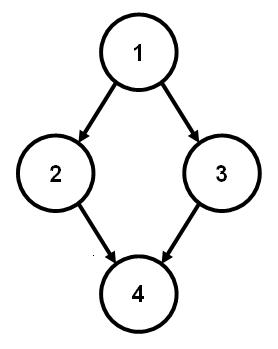
\includegraphics[scale=0.3]{media/digraph2.jpg}
	\caption{Network $\to$ DiGraph}
	\end{figure}
	\end{columns}
	\pause
	\vspace*{20pt}
	Time is discreet\\
	Hardware Limitation : Only 1 message can be sent per link per time unit
\end{frame}

\begin{frame}
\frametitle{Initial Work}
	\framesubtitle{Time-Triggered (TT) schedules}

	\vspace*{-8pt}

	\begin{columns}
	\column{0.5\textwidth}
	\begin{figure}
	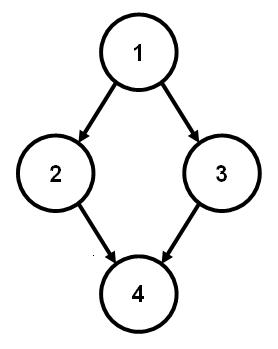
\includegraphics[scale=0.4]{media/digraph2.jpg}
	\caption{Network as a DiGraph}
	\end{figure}

	\column{0.5\textwidth}

	\begin{table}
	\begin{tabular}{c | c | c}
	Message & Source & Target\\
	\hline \hline
	m0 & v1 & v2\\
	m1 & v1 & v4
	\end{tabular}
	\caption{Messages}
	\end{table}

	\vspace*{-15pt}

	\pause

	\begin{table}
	\begin{tabular}{c | c | c}
	Message & Edge & Time\\
	\hline \hline
	m0 & (1-2) & 0\\
	m1 & (1-2) & 1\\
	m1 & (2-4) & 2
	\end{tabular}
	\caption{A Time-Triggered Schedule}
	\end{table}
	\end{columns}


	\pause
	\color{red}

	\vspace*{-15pt}
	\begin{center}
	TT scheduling assumes that the network is fixed, is costly\\
	However, in practice, networks are faulty (discussed later)
	\end{center}
\end{frame}

\begin{frame}
\frametitle{Previous Paper - An Adverserial Approach}
	\begin{itemize}
	\item Time-Triggered Schedules
	\item Simple Error Recovery Protocol %- forward message on some other edge
	\item $(k,l)-resistance$:	\\
	If at most $k$ crashes occur, at least $l$ messages arrive\\[3ex]
	\end{itemize}
	\hspace*{20pt}$ crash $ : A link goes down permanently\\[3ex]
	% \pause
	% Can also be viewed as a saboteur game!\\[2ex]
	\pause
	\color{blue}
	In contrast, we study networks with probablistic faults, addressing multiple types of faults\\
	A more detailed specification ahead...
\end{frame}

\begin{frame}
\frametitle{Handling New Faults}
	\begin{itemize}
	\item Edge faults
	\begin{itemize}
		\item Permanent Crashes
		\pause
		\item Temporary Crashes
	\end{itemize}
	\item Message faults
	\begin{itemize}
		\item Message Delays
		\item Message Losses
		\pause
		\begin{itemize}
			\item Modelled as: Message reappears at a vertex immediately after it was sent from it.\\[2ex]
		\end{itemize}
	\end{itemize}
	\end{itemize}
	\pause
	\begin{center}
	\color{red}
	Things become messy with Time-Triggered Schedules.\\We move to a cleaner notion of message forwarding.
	\end{center}
\end{frame}

\begin{frame}
\frametitle{Forwarding Scheme}
	\framesubtitle{Components}
	% \begin{enumerate}
	\begin{block}{Paths}
	For each message $ m\in M $, specify the possible paths that can be taken by $ m $
	\end{block}
	\pause
	\begin{block}{Priority Scheme}
	Each vertex $ v $ has a total order $ \prec _{v} $ on the set of
	messages $ M $. $$\forall m_1,m_2 \in M,\ m_1\prec _{v}m_2 \implies m_1 \text{ has higher priority over } m_2 \text{ at } v$$
	\end{block}
	\pause
	\begin{block}{Algorithm}
	\textit{Input}: Message queue at a vertex, its active out-going edges\\
	\textit{Output}: The links on which each message is forwarded, if any
	\end{block}
	% \end{enumerate}
\end{frame}

\begin{frame}
\frametitle{Problem Statement}
	\textbf{Given}:
	\begin{itemize}
		\item G, M, t
		\item $p_{crashes}$ = Pr(Edge Fault)
		\item $p_{omission}$ = Pr(Message Fault)
		\item Forwarding Scheme\\[3ex]
	\end{itemize}
	\pause
	\textbf{Find}:
	The score of the Forwarding Scheme, where\\
		$$Score(\text{Forwarding Scheme}) = \Pr(\text{All messages arrive by time t})$$
\end{frame}

% \begin{frame}
% \frametitle{The Different Approaches}
% \begin{enumerate}
% \item Naive Approach (+Optimization)
% \item Bit-Adder
% \item Weighted Model Counting
% \item Monte-Carlo Approach (+Multiprocessing)
% \end{enumerate}
% \end{frame}

% =======================
% The Counting Approach
% =======================

\begin{frame}
\frametitle{The Counting Approach}
	Build a SAT Program : $ f $ that simulates the network\\[2ex]
	Satisfying assignment $\sigma$\ \leftrightarrow\ A fault sequence that leads to a \textit{Bad} outcome\\
	\textit{Bad} outcome: Not all messages arrive on time\\[3ex]
	% \vspace*{-5pt}
	% $$ \sigma \vDash f \implies \neg(\text{All Message Arrive by time t}) $$
	\pause
	\begin{block}{$\ $}
	$$ Score(\text{Forwarding Scheme}) = 1-\sum_{\sigma \vDash f}\Pr(\sigma) $$
	\end{block}
\end{frame}

\begin{frame}
\frametitle{The Counting Approach}
\framesubtitle{Naive}

	SAT Program : $ f $ \\[3ex]
	\textbf{Finding the score}:\\
	Initialize $Score(\text{Forwarding Scheme}):=1$
	\begin{enumerate}
		\item Get a solution $\sigma$
		\item Calculate $\Pr(\sigma)$, subtract it from $Score(\text{Forwarding Scheme})$
		\item Add $\neg \sigma$ to the program as a constraint
		\item Repeat this process until there is no solution left\\[3ex]
	\end{enumerate}
	We have found $Score(\text{Forwarding Scheme})$
	% \pause
	% \color{red}
	% There may be too many solutions!\\
	% A lot of them have negligible probabilities.\\
\end{frame}

\begin{frame}
\frametitle{The Counting Approach} %What is WMC?
\framesubtitle{Weighted Model Counting (WMC)}

	WMC is a generalization of $SAT$ counting.\\
	\begin{block}{WMC}
	Let $f$ be a $SAT$ formula
	% \begin{eqnarray}
		$$WMC(f) = \sum_{\sigma \vDash f}Weight(\sigma)$$
		% $$Weight(\sigma) = \prod_{l \in L}{Weight(l=\sigma(l))}$$
	% \end{eqnarray}
	\end{block}
\end{frame}

\begin{frame}
\frametitle{The Counting Approach} %What is literal-WMC?
\framesubtitle{Literal-WMC [Chakraborty, Kuldeep, Vardi 2015]}

	Each literal $l$\ is assigned a weight s.t.\\
	\vspace*{-5pt}
	$$Weight(l=True) + Weight(l=False) = 1$$\\
	% \vspace*{20pt}
	\begin{block}{WMC}
	Let $\sigma$\ be an assignment to $ f $.
	% \begin{eqnarray}
		% $$WMC(f) = \sum_{\sigma \vDash f}Weight(\sigma)$$
		$$Weight(\sigma) = \prod_{l \in L}{Weight(l=\sigma(l))}$$
	% Thinking of $Weights$ as $Probabilities$,
	% 	$$\ \ \ \ \ \ \ \  = \prod_{l \in L}{\Pr(l=\sigma(l))}$$
	% \end{eqnarray}
	\end{block}
\end{frame}

\begin{frame}
\frametitle{The Counting Approach}
\framesubtitle{Literal-WMC [Chakraborty, Kuldeep, Vardi 2015]}
	SAT formula $ f $\ that simulates the network. (As described earlier)\\[1ex]
	We made certain modifications to $f$, while preserving its one-one correspondence properties, such that
	% % Every crash sequence \mapsto\ a unique assignment \sigma\
	% % $$\sigma \vDash f \iff \text{All Message Arrive by time t}$$
	% % \vspace*{-15pt}
	% \begin{block}{Recall}
	% $$ Score(\text{Priority Scheme}) = \sum_{\sigma \vDash f}\Pr(\sigma) $$
	% % $$\Pr(\sigma) = \prod_{l \in L}{\Pr(l=\sigma(l))}$$
	% \end{block}
	% \pause
	% This is very similar to what Weighted Model Counting offers!
	$$\exists \text{ Weight assignment to all $l \in L$, such that},$$
	$$WMC(f) = 1-Score(\text{Forwarding Scheme})$$
\end{frame}

\begin{frame}
\frametitle{The Counting Approach}
\framesubtitle{WMC \to \ UMC Reduction [Chakraborty, Kuldeep, Vardi 2015]}
	% \begin{block}{WMC}
	% Let $f$ be a $SAT$ formula
	% % \begin{eqnarray}
	% 	$$WMC(f) = \sum_{\sigma \vDash f}Weight(\sigma)$$
	% 	$$Weight(\sigma) = \prod_{l \in L}{Weight(l=\sigma(l))}$$
	% % \end{eqnarray}
	% \end{block}
	% Clearly, WMC can be directly used for models with independent random variables.\\
	% % \vspace*{10pt}
	% % Note that $paper^{2}$ only offers a reduction from WMC problems to Unweighted Model Counting.\\
	% \pause
	% \color{red}
	% Our variables were not independent!\\
	% We had to make modifications to use the WMC to UMC Reduction\footnote{\href{http://ijcai.org/Proceedings/15/Papers/103.pdf}{From Weighted to Unweighted Model Counting}}\\
	\begin{itemize}
		\item We use the WMC \to \ UMC Reduction technique
		\item The problem of Scoring(Forwarding Scheme) has reduced to counting satisfying assignments to a SAT formula
	\end{itemize}
\end{frame}

\begin{frame}
\frametitle{The Counting Approach}
\framesubtitle{UMC Counting}
	To obtain $Score(\text{Forwarding Scheme})$,\\
	We can use any of these counting tools:
	\begin{itemize}
	\item Exact
		\begin{itemize}
		\item SharpSAT\footnote{https://sites.google.com/site/marcthurley/sharpsat}*
		\end{itemize}

	\item Approximate
		\begin{itemize}
		\item Cryptominsat\footnote{https://github.com/msoos/cryptominisat}
		\item ApproxMC [Chakraborty et al 2015]\footnote{https://www.cs.rice.edu/CS/Verification/Projects/ApproxMC/Paper.pdf}\\[3ex]
		\end{itemize}
	\end{itemize}
	*SharpSAT gives the best results
\end{frame}

% ============
% Just for fun
% ============

\begin{frame}
\frametitle{Just for Fun!}
	\begin{figure}
	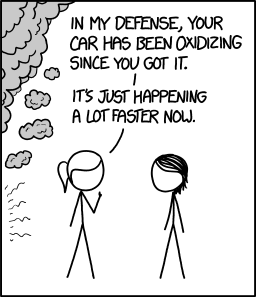
\includegraphics[scale=0.7]{media/xkcd1.png}
	% 
\includegraphics[scale=0.4]{media/fun1.jpg}
	\caption{\tiny Source: xkcd.com}
	\end{figure}
\end{frame}

% ======================
% The Iterative Approach
% ======================

\begin{frame}
\frametitle{The Iterative Approach}
	Build a SAT Program : $ f $ that simulates the network\\[2ex]
	Satisfying assignment $\sigma$\ \leftrightarrow\ A fault sequence that leads to a \textit{Bad} outcome\\
	\textit{Bad} outcome: Not all messages arrive on time\\[3ex]
	\vspace*{-10pt}
	\begin{figure}
	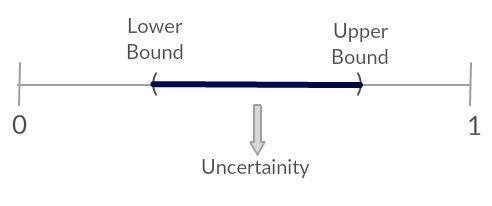
\includegraphics[scale=0.4]{media/Real_Line.png}
	\end{figure}
	\vspace*{-10pt}
	\begin{itemize}
	\item We iteratively examine particular sample spaces to reduce uncertainity
	\item We examine the sample spaces of exactly $k$\ crashes occuring, $k\in\{0,1,2...\}$. We assume fault probabilitites are low.
	\end{itemize}
\end{frame}


\begin{frame}
\frametitle{The Iterative Approach}
	\begin{block}{Additional SMT Constraint in $f$}
	\begin{equation}
		Total\ Number\ of\ crashes = k
	\end{equation}
	\begin{flushright}
		where $k\in\{0,1,2...\}$
	\end{flushright}
	\end{block}
	\pause
	To find $Score(\text{Forwarding Scheme})$,\\
	% Initialize $Score(\text{Forwarding Scheme}):=1$
	\begin{itemize}
	\item For successive $k\in\{0,1,2...\}$
	\begin{enumerate}
		\item Get a solution $\sigma$
		\item Calculate $\Pr(\sigma)$, add it to $\Pr _{temp}$
		\item Add $\neg \sigma$ to the program as a constraint
		\item Repeat this process until there is no solution left
	\end{enumerate}
	\item Update upper,lower bounds on $Score(\text{Forwarding Scheme})$
	\item Stop after reaching enough precision
	\end{itemize}
	We have found $Score(\text{Forwarding Scheme})$
\end{frame}

\begin{frame}
\frametitle{The Iterative Approach}
\framesubtitle{Optimization}
	Identify and add minimal sub-constraint\\[2ex]
	Let $ \sigma \vDash f$\\
	\begin{itemize}
	\item Amongst the crashes occuring at $time=0,1,2,...$,\\
	Find the smallest $t_{doomed}$ such that\\
	Crashes occuring until $t_{doomed}$ are sufficient for $\neg\text{(All messages arrive by t)}$\\
	$$\text{Minimal sub-constraint} = \neg(\text{crashes occuring until }t_{doomed})$$
	\item This is done in practice by building a SMT Program for each $time\in\{0,1,2...\}$, which is UNSAT if Crashes occuring until $t_{doomed}$ are sufficient for $\neg\text{(All messages arrive by t)}$
	\end{itemize}
\end{frame}

\begin{frame}
\frametitle{The Iterative Approach}
\framesubtitle{Bit-Adder Approach}
	SAT formula $ f $\ that simulates the network. (As described earlier)\\[1ex]
	\begin{block}{Recall the only SMT Constraint...}
	$$Total\ Number\ of\ crashes = k$$
	\begin{flushright}
		where $k\in\{0,1,2...\}$
	\end{flushright}
	\end{block}

	\pause

	\begin{itemize}
	\item We simulate the execution of a bit-adder circuit
	\item Hence, convert this SMT constraint to a SAT constraint
	\item We now have a purely SAT formula
	\item Use a SAT counting tool
	\item Update probability bounds
	\end{itemize}
	Note: There is little work on counting satisfying assignments to SMT formulas
\end{frame}

\begin{frame}
\frametitle{Monte-Carlo}
	Given $\epsilon \ and\ \delta$,\\
	Report $Score(\text{Priority Scheme})$ within an error $\epsilon$\ with a confidence $1-\delta$.\\[2ex]
	This is based on the Hoeffding's inequality.\\[2ex]
	Method:
	\begin{itemize}
	\item Simulate the network $n$\ times, randomly deciding faults
	\item Amongst the $n$\ trials, $k$\ trials are successful
	\item $Score(\text{Priority Scheme}) \approx \frac{k}{n}$
	\item Use multiprocessing for faster results
	\end{itemize}
\end{frame}

\begin{frame}
\frametitle{Results}
\framesubtitle{Scaling}

	Settings with the following sizes can be solved within 45 minutes:

	\begin{table}
	\begin{tabular}{l | c | c | c | c}
	Approach & Edges & Nodes & Messages & Timeout\\
	\hline \hline
	Naive & 17 & 7 & 7 & 7\\
	Naive+Opt & 17 & 7 & 7 & 7\\
	WMC & 20 & 8 & 8 & 8\\
	Bit-Adder & 22 & 9 & 9 & 9\\
	Monte-Carlo* & 80 & 32 & 32 & 32\\
	Monte-Carlo Threaded*$^{\dagger}$ & 112 & 45 & 45 & 45\\
	\end{tabular}
	\caption{Problem Scaling}
	\end{table}
	% $\\ \\$
	*$\ \epsilon=0.01, \delta=0.001$\\
	$^{\dagger}$\ 4 threads on a quad-core machine
\end{frame}

\begin{frame}
\frametitle{Results}
\framesubtitle{Monte Carlo Runtime}
	\vspace*{-10pt}
	\begin{figure}
	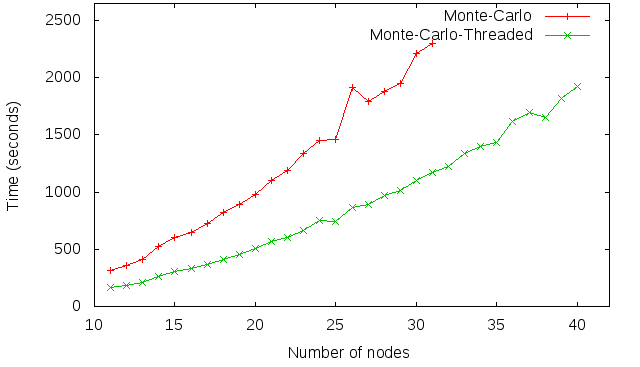
\includegraphics[scale=0.5]{media/monte_carlo_runtime.png}\\
	% \caption{Monte Carlo Run Time*$^{\dagger}$}
	\end{figure}
	% $ \ \\ \ $
	\vspace*{-20pt}
	\tiny{*$\ \epsilon=0.01, \delta=0.001$\\
		$^{\dagger}$\ 4 threads on a quad-core machine}
\end{frame}

\begin{frame}
\frametitle{What Next?}
	\begin{itemize}
	\item Find good \textit{Forwarding Schemes}
		\begin{itemize}
		\item Heuristics
		\item Improving Priority Schemes
		\end{itemize}
	\item Finding Complexity Bounds
		\begin{itemize}
		\item Prove complexity bounds for these problems
		\end{itemize}
	\end{itemize}
\end{frame}

\begin{frame}
\frametitle{Thank You}
% Questions?
% \Large{Questions?}
\end{frame}

\end{document}

% \begin{frame}
% \frametitle{Bib}

% \begin{thebibliography}{5}
% \bibitem{prev_paper}
% Guy Avni, Shibashis Guha and Guillermo Navas-Rodriguez.
% \textit{Synthesizing Time-Triggered Schedules for Switched Networks with Faulty Links}.
% Submitted

% \bibitem{WMC}
% Supratik Chakraborty, Dror Fried, Kuldeep S. Meel and Moshe Y. Vardi.
% \textit{From Weighted to Unweighted Model Counting}.
% IJCAI

% \bibitem{SharpSAT}
% SAT Counting,
% \\\texttt{https://sites.google.com/site/marcthurley/sharpsat}

% \bibitem{Cryptominsat}
% Approximate SAT Counting,
% \\\texttt{https://github.com/msoos/cryptominisat}

% \bibitem{ApproxMC}
% Supratik Chakraborty, Kuldeep S. Meel and Moshe Y. Vardi.
% \textit{A Scalable Approximate Model Counter}.
% \\\texttt{https://bitbucket.org/kuldeepmeel/approxmc}

% \end{thebibliography}

% \end{frame}

% \begin{frame}[allowframebreaks]
% \frametitle{References}
% 	\bibliographystyle{amsalpha}
% 	\bibliography{ref.bib}
% \end{frame}

% CITATIONS
% =========
% Synthesizing Time-Triggered Schedules for Switched Networks with Faulty Links
% Authors: Guy Avni, Shibashis Guha, and Guillermo Navas-Rodriguez
% Status: Submitted

% From Weighted to Unweighted Model Counting
% Authors: Supratik Chakraborty, Dror Fried, Kuldeep S. Meel, Moshe Y. Vardi
% \href{http://ijcai.org/Proceedings/15/Papers/103.pdf}

% SharpSAT
% \href{https://sites.google.com/site/marcthurley/sharpsat}

% Cryptominsat
% \href{https://github.com/msoos/cryptominisat}

% ApproxMC
% A Scalable Approximate Model Counter
% Authors: Supratik Chakraborty, Kuldeep S. Meel, Moshe Y. Vardi
% \href{https://www.cs.rice.edu/CS/Verification/Projects/ApproxMC/Paper.pdf}
